\documentclass[10pt,a4paper]{article}
\usepackage[a4paper,margin=1.8cm,top=1.5cm,bottom=1.6cm]{geometry}
\usepackage[T1]{fontenc}
\usepackage{lmodern}
\usepackage{microtype}
\usepackage{amsmath,amssymb}
\usepackage{booktabs}
\usepackage{graphicx}
\usepackage{xcolor}
\usepackage[hidelinks]{hyperref}
\usepackage{enumitem}
\usepackage{titlesec}
\usepackage{caption}
\usepackage[most]{tcolorbox}
\setlist{nosep,leftmargin=1.2em}
\titleformat{\section}{\normalfont\large\bfseries}{\thesection}{0.6em}{}
\titlespacing*{\section}{0pt}{1.1ex}{0.5ex}
\captionsetup{font=small,skip=3pt}
\setlength{\parindent}{0pt}
\setlength{\parskip}{0.5ex}
\setlength{\abovedisplayskip}{4pt}\setlength{\belowdisplayskip}{4pt}
\setlength{\abovedisplayshortskip}{2pt}\setlength{\belowdisplayshortskip}{2pt}

\begin{document}

{\large\bfseries IE 425 Data Mining $\cdot$ Fall 2026 $\cdot$ Term project checkpoint}\\[0.3ex]
{\bfseries Forecasting daily bike arrivals in Oslo} \hfill Group 11 $\cdot$ 6 November 2026\\[0.2ex]
{\small Ahmet Burak Ekin (2021401141), Ömer Osman Oğultürk (2021402216), Mustafa Talha Aydın (2022402192)}

\vspace{-0.6ex}\noindent\rule{\linewidth}{0.4pt}

%==============================================================================
\section{How we frame the problem}

\textbf{Unit of analysis.} One \emph{cluster-day}: a pair $(i,d)$ of a station cluster
$i\in\{1,\dots,5\}$ (Center, East, North, North-west, West) and an Oslo calendar day $d$
(00:00--23:59, Europe/Oslo). Each target day contributes five rows.

\textbf{Target.} The inflow of cluster $i$ on day $d$,
\[
  y_{i,d} \;=\; \sum_{s\in \mathcal{S}_i} a_{s,d},
\]
where $\mathcal{S}_i$ is the set of scored stations assigned to cluster $i$ in
\texttt{stations.csv} (fixed for the term) and $a_{s,d}$ is the number of cleaned trips that
\emph{end} at station $s$ on Oslo day $d$. The trip files are in UTC and are converted with the
Europe/Oslo time zone, never a fixed offset. A closed station contributes $0$. The forecast
$\hat y_{i,d}\ge 0$ is a real number.

\textbf{Origin and what is known there.} Day $d$ is forecast at the origin $t_0(d)=$ 21:00 Oslo
time on day $d-1$, so the horizon runs from 3 to 27 hours ahead. At $t_0(d)$ we may use:
\begin{itemize}
  \item complete daily counts $y_{i,t}$ for $t\le d-2$ (\texttt{cluster\_daily});
  \item the \emph{partial} count of day $d-1$, trips that ended before 21:00, written $e_{i,d-1}$
        (\texttt{cluster\_before21}); in October--December this is about 92\% of a day;
  \item the calendar of $d$ (weekday, public holidays), known in advance;
  \item weather \emph{forecasts} for $d$ issued before $t_0(d)$ (\texttt{source="forecast"});
        measured weather only for whole days up to about $d-3$.
\end{itemize}
We may \emph{not} use the whole-day count of $d-1$, trips that end after 21:00 on $d-1$, or the
actual weather of $d$: each of these is leakage. Training rows and the prediction row are built by
the same code with the same as-of cut.

\textbf{Success criterion.} Over the five clusters and the $D$ target days of a round,
\[
  \mathrm{WMAPE} = \frac{\sum_{i=1}^{5}\sum_{d=1}^{D}\lvert y_{i,d}-\hat y_{i,d}\rvert}
                        {\sum_{i=1}^{5}\sum_{d=1}^{D} y_{i,d}},
  \qquad
  \text{bias} = \frac{\sum_{i,d}\hat y_{i,d}}{\sum_{i,d} y_{i,d}},
  \qquad
  \text{skill} = 1-\frac{\mathrm{WMAPE}}{\mathrm{WMAPE}_{B1}} .
\]
A model is useful to us only if it beats the yardstick B1 (skill $>0$) by more than the
year-to-year noise, with a bias near $1.00$. WMAPE weights each cluster by its volume, so the
Center (about 54\% of the inflow) dominates the score. The clusters' errors are strongly
correlated (about 0.85), so a round of 9--12 days is worth little more than 9--12 independent
forecasts; we treat differences of about $0.02$ in WMAPE as noise.

\textbf{Assumptions we check.}
(i) \emph{Level shifts}: 2019 was about twice as busy as 2023--2025 and 2026 is about 8\% above
2025, so old years may hurt rather than help.
(ii) \emph{Seasonality}: the rounds fall in the steepest part of the autumn decline, and the outer
clusters fall faster than the Center.
(iii) \emph{Weekday structure} and (iv) \emph{weather} (24~mm of rain on 8~October 2026 halved the
city inflow).
(v) \emph{Stations} open and close, which moves a cluster's level slowly.
(vi) \emph{Clock}: daylight-saving days have 23 or 25 hours; all test days are ordinary.

%==============================================================================
\section{Validation plan}

\textbf{Rolling origin, replaying the harness.} For every validation day $d$ we rebuild the
information set as it stands at $t_0(d)$ (full days up to $d-2$, the before-21:00 count of
$d-1$) and produce one forecast. Anything that is estimated (shares, factors, model coefficients)
uses only data that was available at that origin, as \texttt{fit\_model} does in the real run.

\textbf{Folds: the test calendar in past years.} The rounds are 9--20~November (R1, 12 days) and
23~November--1~December (R2, 9 days). We replay these two windows in 2022, 2023, 2024 and 2025:
eight folds, 84 target days, 420 cluster-days. We do not validate on 2019--2021 (a level twice as
high in 2019, the closure from 9~December~2019 to 17~March~2020, winter shutdowns before 2021),
but a model may still use those years for training.

\textbf{Three-way split in time.} Features, settings and hyper-parameters are chosen on the
2022--2024 folds (\emph{tune}). The 2025 folds, closest to the current regime, are the
\emph{check}: each candidate is scored there once, after its settings are fixed. We report every
fold, because one year's November can be easy and the next one hard.

\textbf{Sanity checks.}
(a) On 8~October--16~December of 2022--2025 our code reproduces the brief's yardsticks:
WMAPE $0.252$ for last week's value and $0.204$ for B1 (bias $1.117$), and all five per-cluster
values to two decimals. This checks our data, time zones and the implementation of B1.
(b) We also score 8~October--5~November 2026, the only weeks of the current, higher level.
(c) The submitted file is run through the self-check kit on several cut dates
(\texttt{selfcheck.py --cut-at}) to verify the two-function contract, the 15-minute and 6~GB
limits, and that the weather it requests is present.

%==============================================================================
\section{First baseline and its validation score}

\textbf{Yardstick B1.} With complete days up to $d-2$ only,
\[
  \hat y^{B1}_{i,d} \;=\;
  \underbrace{\tfrac14\bigl(y_{i,d-7}+y_{i,d-14}+y_{i,d-21}+y_{i,d-28}\bigr)}_{F_{i,d}:\ \text{same weekday, last four weeks}}
  \times
  \underbrace{\frac{\tfrac17\sum_{k=2}^{8} y_{i,d-k}}{\tfrac1{28}\sum_{k=2}^{29} y_{i,d-k}}}_{r_{i,d}:\ \text{recent level}},
\]
with $r_{i,d}=1$ when the 28-day mean is zero. The naive alternative is last week's value,
$\hat y_{i,d}=y_{i,d-7}$.

\textbf{First improvement: B1-evening $\times$ seasonal factor.} Two changes, both using only
what is known at the origin.
\emph{(1) Use the evening of $d-1$.} The share of a day that arrives before 21:00 is estimated from
the last eight complete days with the same weekday as $d-1$,
$\hat p_{i,d-1}=\tfrac18\sum_{k=1}^{8} e_{i,d-1-7k}/y_{i,d-1-7k}$, and the whole of $d-1$ is
estimated as $\tilde y_{i,d-1}=e_{i,d-1}/\hat p_{i,d-1}$. The level ratio then includes that day:
\[
  \tilde r_{i,d} = \frac{\tfrac17\bigl(\tilde y_{i,d-1}+\sum_{k=2}^{7}y_{i,d-k}\bigr)}
                        {\tfrac1{28}\bigl(\tilde y_{i,d-1}+\sum_{k=2}^{28}y_{i,d-k}\bigr)},
  \qquad
  \hat y^{E}_{i,d} = F_{i,d}\,\tilde r_{i,d}.
\]
\emph{(2) Correct the seasonal over-forecast.} A trailing level ratio lags behind the November
decline, so B1 forecasts too many bikes (Figure~1b). For a day $d$ in year $Y$ we take the realised
ratios $y_{i,t}/\hat y^{E}_{i,t}$ of \emph{earlier} years only, on days $t$ within $\pm h$ days of the
same calendar date (days on which the whole system was closed are left out), and use their median:
\[
  c_i(d)=\operatorname*{median}\Bigl\{\,y_{i,t}/\hat y^{E}_{i,t}\;:\; t\in\text{years }2019,\dots,Y-1,\ \lvert t-d^{(t)}\rvert\le h\Bigr\},
  \qquad
  \hat y_{i,d}=c_i(d)\,\hat y^{E}_{i,d},
\]
where $d^{(t)}$ is the date $d$ moved to the year of $t$. The half-width $h=14$ days was chosen on
the tune folds from $\{3,5,7,10,14,21,28\}$; the 2025 folds were scored once afterwards.

\begin{table}[h]
\centering\small
\caption{WMAPE and bias (forecast/actual) of each model; skill against B1 over all 84 days.
Tune = 2022--2024 folds (36 R1 days, 27 R2 days); check = 2025 folds.}
\label{tab:res}
\setlength{\tabcolsep}{3.5pt}
\begin{tabular}{@{}l cc cc cc cc cc c@{}}
\toprule
 & \multicolumn{2}{c}{R1 tune} & \multicolumn{2}{c}{R2 tune} & \multicolumn{2}{c}{R1 2025} & \multicolumn{2}{c}{R2 2025} & \multicolumn{2}{c}{All 84 days} & \\
\cmidrule(lr){2-3}\cmidrule(lr){4-5}\cmidrule(lr){6-7}\cmidrule(lr){8-9}\cmidrule(lr){10-11}
Model & WMAPE & bias & WMAPE & bias & WMAPE & bias & WMAPE & bias & WMAPE & bias & skill \\
\midrule
Last week's value & 0.208 & 1.05 & 0.419 & 1.33 & 0.255 & 1.20 & 0.321 & 1.26 & 0.272 & 1.15 & $-0.29$ \\
B1 (yardstick) & 0.166 & 1.08 & 0.305 & 1.27 & 0.201 & 1.19 & 0.272 & 1.23 & 0.211 & 1.15 & 0 \\
B1 $\times$ seasonal factor & 0.140 & 0.95 & 0.222 & 1.04 & 0.122 & 1.05 & 0.204 & 1.00 & 0.160 & 0.99 & $+0.24$ \\
B1-evening $\times$ seasonal factor & 0.131 & 0.95 & 0.208 & 1.01 & 0.107 & 1.05 & 0.211 & 0.99 & 0.150 & 0.98 & $+0.29$ \\
\bottomrule
\end{tabular}
\end{table}

\begin{figure}[h]
\centering
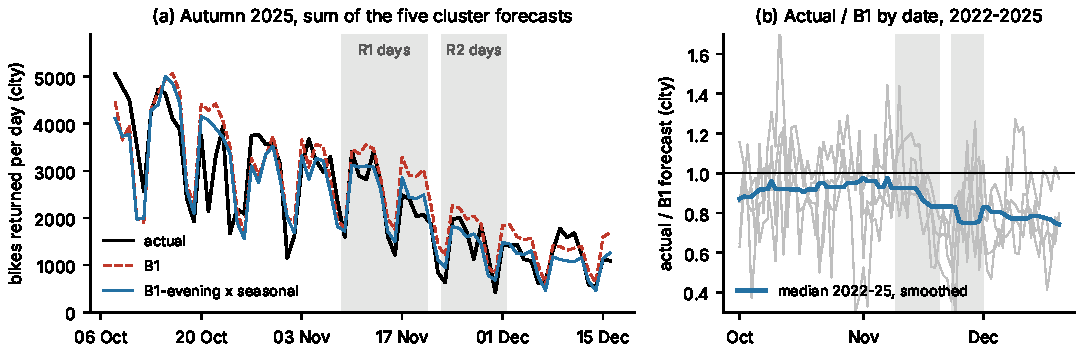
\includegraphics[width=\linewidth]{fig1.pdf}
\caption{(a) City inflow in autumn 2025 (sum over the five clusters) with the B1 forecast and our
first model; gray bands are the round windows replayed in 2025. (b) Ratio of actual inflow to the
B1 forecast for each year 2022--2025 (gray) and its smoothed median (blue): below 1 through
November, deepest in the R2 window.}
\end{figure}

\textbf{What the numbers support.}
B1's error in November is largely systematic: its bias is 1.08 on the R1 tune days and 1.27 on
the R2 tune days. The seasonal factor removes most of it (bias 0.95--1.05) and lowers WMAPE over
the 84 days from 0.211 to 0.160; adding the evening of $d-1$ lowers it to 0.150 (skill $+0.29$).
Per cluster, the North-west stays the hardest (WMAPE 0.194 against 0.289 for B1) and the Center
the easiest (0.133 against 0.185). The spread across years is large: the eight folds range from
0.06 to 0.26 for our model and from 0.13 to 0.38 for B1, so the gain from the evening term
(0.010) is within the noise band and must keep showing up before we rely on it. On
8~October--5~November 2026 the gain is smaller (B1 0.247, our model 0.231): in October the
decline is mild and the day-to-day swings come from the weather, which neither model sees.

%==============================================================================
\section{Next steps}
\begin{enumerate}
  \item \textbf{Freeze 1 (8 November).} Submit B1-evening $\times$ seasonal factor as
        \texttt{main.py}: \texttt{fit\_model} estimates $c_i(\cdot)$ and $\hat p$ from the
        snapshot, \texttt{make\_forecast} applies them, with a fall-back to B1 if a value is
        missing. Checked with the self-check kit before every push.
  \item \textbf{Weather.} Request hourly precipitation and temperature \emph{forecasts} at the five
        cluster centres (archive from January 2025), aggregate them to Oslo-day features
        (daytime rain, mean temperature), and model the remaining log-ratio
        $\log(y_{i,d}/\hat y_{i,d})$. We train on forecasts, not on measured weather, so that the
        training rows match the prediction row.
  \item \textbf{A learned model.} A regularised regression and a gradient-boosted tree on the log
        scale (lags, level ratios, weekday, day of year, weather), with an absolute-error loss
        that matches WMAPE; one model per cluster against one pooled model, and a bottom-up sum
        of station forecasts. Each is compared on the same folds and kept only if it beats the
        current model on the tune folds by more than the noise band.
  \item \textbf{The 2026 regime.} Check whether factors learned from 2019--2025 still hold at the
        higher 2026 level, especially for the fast-growing North and North-west clusters.
\end{enumerate}

%==============================================================================
\section*{AI Use Note}
\textbf{Tools.} Claude (Anthropic), used in the Claude desktop app with read access to the course
files, the project brief and the self-check kit.
\textbf{What we asked.} To summarise the brief's and the kit's rules; to write the backtest code
(B1, last week's value, the seasonal and evening variants on the replayed windows) and the figure;
to draft the text of this checkpoint.
\textbf{What we changed.} \textcolor{red}{[2--3 sentences chosen from the box below]}

\begin{tcolorbox}[enhanced, breakable, colback=red!2, colframe=red!55!black, boxrule=0.6pt,
  arc=2pt, left=6pt, right=6pt, top=4pt, bottom=4pt, fontupper=\small,
  title={\small\bfseries TASLAK -- grup i\c{c}in \"{o}neriler. Teslimden \"{o}nce bu kutuyu silin.}]
Yaln\i zca \textbf{ger\c{c}ekten yapt\i\u{g}\i m\i z} \c{s}eyleri se\c{c}ip d\"{u}zenleyelim; 2--3 c\"{u}mle yeter.
Hocan\i n en \c{c}ok de\u{g}er verdi\u{g}i not somut ve kontrol edilebilir olan\i d\i r: neyi kontrol ettik,
neyi yanl\i\c{s} ya da eksik bulduk, neyi neden de\u{g}i\c{s}tirdik. ``Metni okuduk'' gibi genel bir c\"{u}mle
tek ba\c{s}\i na zay\i f kal\i r. Her se\c{c}ene\u{g}in yan\i nda, onu do\u{g}ru k\i lmak i\c{c}in yap\i lmas\i\ gereken i\c{s} yaz\i yor.

\smallskip
\textbf{(A) Kendi c\"{u}mlelerimiz.} \emph{Yap\i lacak: 1.\ b\"{o}l\"{u}m\"{u} brief'in 1.2 ve 2.2 b\"{o}l\"{u}mleriyle
kar\c{s}\i la\c{s}t\i r\i p kendi c\"{u}mlelerinizle yeniden yaz\i n.}\\
``We rewrote Section~1 in our own words after checking each item of the information set against
Sections~1.2 and~2.2 of the brief, and we added [\dots] ourselves.''

\smallskip
\textbf{(B) Elle do\u{g}rulama.} \emph{Yap\i lacak: durum \"{o}zetindeki al\i\c{s}t\i rmay\i\ hesap makinesiyle
yap\i n.}\\
``We recomputed B1 and our forecast by hand for the Center cluster on 13~November 2025 (1926.4 and
1753.3 against an actual 1916) and matched the code. The same example showed us that a model that is
better over 84 days can still lose to B1 on a single day.''

\smallskip
\textbf{(C) Kendi sordu\u{g}umuz bir test.} \emph{Yap\i lacak: bir varsay\i ma itiraz edin. Testi ben
\c{c}al\i\c{s}t\i r\i r\i m, karar\i\ siz verirsiniz.}\\
``We questioned whether 2019, a year twice as busy and closed from 9~December, should enter the
seasonal factor. Dropping it changed the tune-fold WMAPE from [x] to [y], which is within the noise
band, so we [kept / dropped] it.''

\smallskip
\textbf{(D) Fazla iddial\i\ bir ifadeyi d\"{u}zeltmek.} \emph{Yap\i lacak: okurken abart\i l\i\ buldu\u{g}unuz
bir c\"{u}mleyi i\c{s}aretleyin.}\\
``We changed `[\dots]' to `[\dots]' because the 84 validation days do not support the stronger
claim.''

\smallskip
\textbf{(E) Bir \"{o}neriyi reddetmek.} \emph{Yap\i lacak: AI'n\i n \"{o}nerdi\u{g}i bir \c{s}eyi gerek\c{c}eyle
reddettiyseniz yaz\i n.}\\
``We did not adopt the assistant's suggestion to [\dots] because [\dots].''
\end{tcolorbox}

\textbf{What we verified.} Our B1 and last-week scores reproduce the brief's yardstick (0.204 and
0.252, bias 1.12, all per-cluster values to two decimals); summing \texttt{station\_day\_arrivals}
over each cluster's stations gives \texttt{cluster\_daily\_inflow} exactly; every forecast for
day $d$ is built from data available at 21:00 on $d-1$ (shifts checked in the code); and $h$ was
chosen on the 2022--2024 folds before the 2025 folds were scored. Our \texttt{main.py}, run
through the self-check kit at three past origins, gives exactly the forecasts of the backtest.

\end{document}
